\chapter{Problem statement}\label{ch:problem}

Currently there is no way of testing the full chain of devices towards and including an application to their limits without spending a lot of money on dedicated commercial load testing products.
Since today servers can be equipped with 40 and 100Gb/s Network Interface Cards (NICs), the OS and the application that is running on top of the OS should be able to process the amount of traffic that comes in from the NIC.

Testing the entire infrastructure using dedicated commercial equipment for every new service is costly and unpractical.
Nikhef is constantly upgrading infrastructure devices to provide the increasing demands of bandwidth. Currently they rely on the hardware specification from the vendors. 
Engineers at Nikhef have a need to find the limitations of the hardware before they put it into production without spending a lot of money and without depending on special commercial hardware.
 
A wide variety of tools is available to generate traffic. Nikhef is interested in TCP traffic specifically.  
Some of the tools are able to setup TCP sessions to transfer data. But what tool is best used for specific application testing?   
Nikhef wants the ability to test hardware they might buy up to the OSI application layer (layer 7) if applicable. 
Until now they are not able to go beyond the transport layer (layer 4).

\section{Session based}\label{sec:sessionbased}
When sending data over UDP, data gets generated and is transported to the destination. 
If the destination IP port is open the data will be forwarded to the application listening on that specific port.
When the destination does not listen on that specific IP port the data will be discarded. 
 
TCP guarantees the delivery of the data as long as the session is alive between the end nodes.
The session needs to be created before data can be exchanged, a three way handshake between source and destination is performed in order to synchronize settings. 
Guaranteed delivery is done by acknowledging received data and resending unacknowledged data. 
Other techniques like Flow control, Congestion control, and fast retransmission of packets ensure that data is delivered in time and offered to the higher layer protocol in the correct order. 
These techniques all require resource reservation at the client and the server, but also at stateful devices along the path between client and server. 

The technique's implemented in TCP all require buffers to store data until the data is acknowledged by the receiving end.
The buffer sizes are reserved by the OS per sessions and negotiated during the three way handshake.  
When the amount of new sessions is higher than the amount of sessions that get closed due to a time-out or a finish statement, server resources are depleted.

When it comes to layer 7 protocols like HTTP, more resources need to be reserved. HTTP sessions, HTTP state and application state need to be saved. Get requests need to be processed, a response needs to be generated and sent over the session to the user. Normally a web server will cache files that are requested for a specific time using up valuable memory. Hosting a dynamic web page requires the web server to generate the page on request which makes the CPU utilization higher than just hosting a static web site. 

\section{Specifications}\label{sec:specifications}
For the design of tests and the interpretation of the results, specific technical constraints in the 'real world' operating environment and several key implementation parameters are important for this project.

\paragraph{Overloading}\label{par:overload}\mbox{}\\
All the techniques used by TCP make sure an Ethernet link will not be overloaded with congestion as a result. 
In order to find the weakest link in the path towards a service, data should be send using the expected maximum capacity of the devices in the path.
When client and server are connected with 40Gb/s interfaces. One should send data using the full capacity of the links.
This could result in overloading a device in the path, this immediately shows that the intermediate device is the weakest link.

When data can be send at the links full capacity, there might be other limitations in the hardware used in the path.  
For systems administrators it is important for monitoring purposes that these limitations are known.

\paragraph{Throughput}\label{par:throughput}\mbox{}\\
Throughput is the most significant value for generating load: how to best utilize the total capacity of a link. When using TCP the header causes 12 bytes more overhead in comparison to a UDP header (a UDP header is 8 bytes). But in return TCP offers techniques that will not overload a device. 

\paragraph{Packet size}\label{par:packetsize}\mbox{}\\
Ethernet is used during this research, therefore all references to packet sizes are based on Ethernet standards\cite{ethernet_frame_2017} with IP and TCP headers included.
Due to collision detection the minimum payload inside an Ethernet frame is 46 bytes.
The Ethernet frame and the payload combined have a minimum size of 64 bytes. 
A VLAN tag is excluded which adds 4 bytes.
A packet is always preceded with a 8 byte preamble.
An Inter Frame Gap between the packets is used to separate the packets. This is a 12 byte gap. 
This makes a total of at least 88 bytes of data from the beginning of a packet to the beginning of a new packet. Figure \ref{fig:juniperethernetframe} gives a representation of an Ethernet packet. 

\begin{figure}[H]
  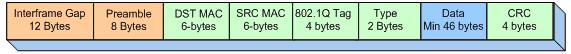
\includegraphics[scale=1]{images/ethernetframe.jpg}
  \caption{Representation of an Ethernet frame used during this report.}
  \label{fig:juniperethernetframe}
\end{figure}

\paragraph{Packets per second}\label{par:pps}\mbox{}\\
When a link has a speed of 40Gb/s and packets have a minimum size of 88bytes (which includes the inter frame gap, the preamble the data link frame and a VLAN tag) a maximum of 56.8 Million packets per second (Mpps) can be transferred over the link in one direction. When using a 100Gb/s line the theoretical maximum is 142 Mpps.   

\paragraph{Sessions}\label{par:sessions}\mbox{}\\
A TCP session is a unique tuple of source IP, destination IP, source port and destination port. An established session may involve more than one message in each direction.
The amount of sessions per second is a determining factor for the availability of services behind firewalls. A firewall needs to keep track of the states of the sessions from source to destination. 
When new sessions to a server are opened, the firewall has to process them according to the rule base. When a session is approved, most vendors move it to fast-path processing. 
This is a table with accepted sessions, allowing traffic in the same session to be handled in hardware. This means that only the first packet of a new session is handled in the slow-path and the limitations of a firewall can be found in the amount of new sessions per second.

\paragraph{Application specific traffic}\mbox{} \\
According to Sandvine\cite{phenomena_2017},(a global communications solutions service provider that published bi-annual traffic baseline reports), around 70\% of the traffic is streaming audio and video. 
Dynamic Adaptive Streaming over HTTP (DASH)\cite{dash} is used to stream video and audio over HTTP. Netflix uses DASH to deliver content to the users. You Tube is accessible over HTTP.
This makes HTTP a suited protocol to use for layer 7 tests during the research.  

\paragraph{Packet size}\label{par:packetsize}\mbox{}\\
According to Murray et all. \cite{murray2012state}  in 2012, 99\% of the traffic inside a corporate network has an MTU size of maximum 1500 bytes. When using Jumbo packets\cite{alliance_2017} (Best practice is an MTU of 9000 bytes towards clients\cite{jet}) the amount of overhead is less because more data can go into on packet. 
More data inside a packet results in less packets. Therefore, less system overhead during the transfer of data. 
Jumbo packets are helpful when large amounts of data need to be transfered between 2 nodes.  
Jumbo packets are not used during the project because according to Murray et all. less than one percent of transferred data has an MTU larger than 1500 bytes. 
Exceptions can be made during a test to see if hardware limits can be reached.

\section{Research question}\label{sec:researchquestion}
The problem statement and the specifications lead to the following research question.

\begin{center}
\textit{What is needed to perform high bandwidth session based throughput tests and how to go beyond pure network infrastructure testing?} \\
\end{center}
The term "high bandwidth" references to at least 40Gb/s. \\
The term "session based" references to TCP traffic. \\

